%!TEX root=../GaugeCNNTheory.tex


\section{مقدمه}


\begin{figure}
	\centering
	\vspace*{-2ex}
	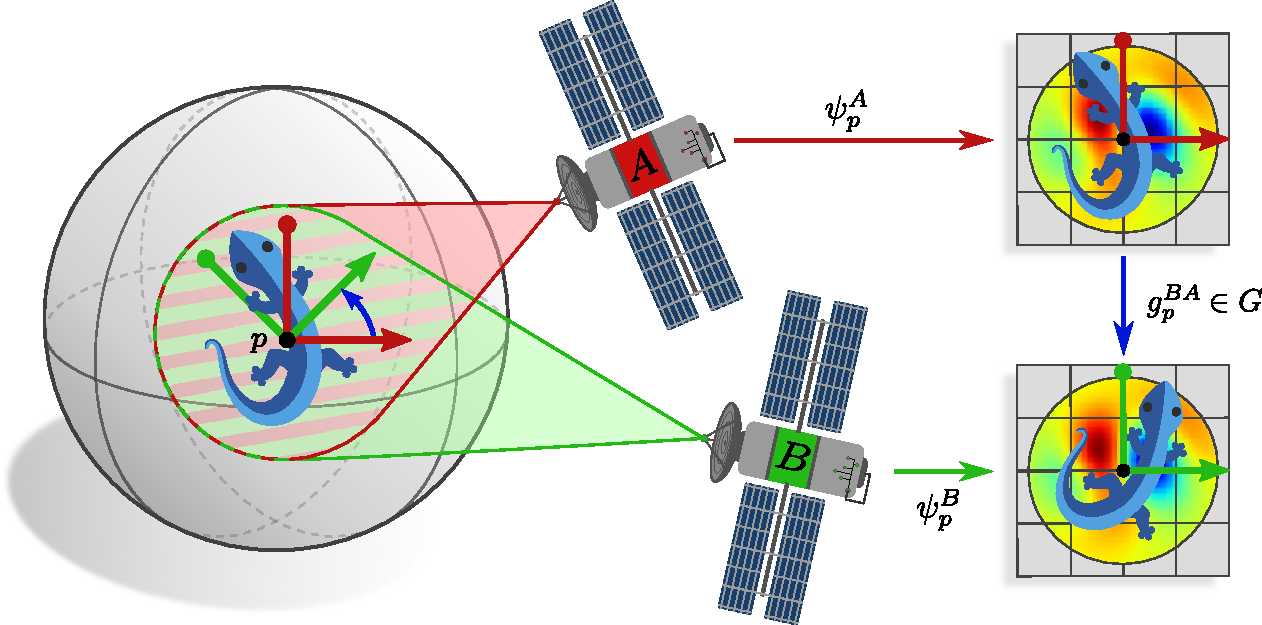
\includegraphics[width=.94\textwidth]{figures/satellite_kernels.pdf}
	\caption{\small
		مشاهده‌گران مختلف $A$ و $B$ ممکن است یک الگوی از ویژگی‌ها را از «دیدگاه» متفاوتی درک کنند.
		ماهواره‌ها در کاربرد ما کرنل‌های کانولوشنی هستند که میدان دید محلی خود را در اطراف~$p$ به یک بردار ویژگی در~$p$ خلاصه می‌کنند.
		«دیدگاه» آن‌ها انتخاب یک چارچوب مرجع محلی (گیج) در~$p$ است که کرنل بر اساس آن تراز می‌شود.
		از آنجا که مشاهدات هر دو دیدگاه نشان‌دهنده یک الگوی یکسان هستند، پاسخ‌های کرنل باید حاوی اطلاعات معادل باشند، یعنی استنتاج باید \emph{مستقل از مختصات} باشد.
		این امر کرنل‌های کانولوشنی را ملزم می‌کند تا تحت \emph{تبدیل‌های گیج محلی} (یعنی تغییرات چارچوب‌های مرجع) \emph{تناوب‌پذیر} باشند.
		سطح تناوب‌پذیری گیج توسط \emph{گروه ساختار}~$G$ تعیین می‌شود، که هم به منیفولد و هم به کاربرد بستگی دارد.
		{\\
			\color{gray}
			\lr{\scriptsize
			(Lizards adapted under the Creative Commons Attribution 4.0 International
			\href{https://github.com/twitter/twemoji/blob/gh-pages/LICENSE-GRAPHICS}{\underline{license}}
			by courtesy of Twitter.)}
		}
	}
	\label{fig:satellite}
\end{figure}


در سال‌های اخیر، شبکه‌های عصبی عمیق به مدل‌های منتخب برای طیف گسترده‌ای از وظایف در یادگیری ماشین تبدیل شده‌اند.
موفقیت مدل‌های عمیق اغلب ریشه در طراحی وظیفه-خاص دارد که منعکس‌کننده ساختار ریاضی داده‌های مورد پردازش است.
یک مثال برجسته شبکه‌های کانولوشنی (\CNNs) هستند که از طریق اتصال محلی و اشتراک وزن فضایی، ساختار مکانی داده‌ها را بهره‌برداری می‌کنند.
از آنجا که یک کرنل یکسان در هر نقطه از فضا اعمال می‌شود، شبکه‌های کانولوشنی نسبت به انتقال تناوب‌پذیر هستند، به این معنی که الگوهای آموخته‌شده را به طور خودکار بر روی موقعیت‌های فضایی تعمیم می‌دهند.
با توجه به موفقیت تجربی قابل توجه \CNNهای اقلیدسی، علاقه زیادی به تعمیم مدل‌های کانولوشنی برای پردازش سیگنال‌ها در دامنه‌های عمومی‌تر و تناوب‌پذیر ساختن آن‌ها تحت گروه‌های تقارن بزرگ‌تر وجود دارد.


این کار به بررسی تعمیم شبکه‌های کانولوشنی به \emph{منیفلدهای ریمانی} می‌پردازد.
یک پیچیدگی عمده در تعمیم شبکه‌های کانولوشنی از فضاهای اقلیدسی $\R^d$ به منیفلدهای ریمانی عمومی این است که \emph{منیفلدهایی دارای انتخاب مرجع جهت ارجح نیستند} که کرنل کانولوشن بتواند بر اساس آن برای اندازه‌گیری ویژگی‌ها تراز شود.
از آنجا که هیچ جهت مرجعی ترجیح داده نمی‌شود، کرنل باید به صورت \emph{دلخواه} بر روی منیفولد تراز شود.
موضوع اصلی این کار تنظیم این اختیار با مستقل ساختن استنتاج شبکه‌ها از تراز خاص کرنل‌های کانولوشن است.
مشخص می‌شود که این امر مستلزم آن است که کرنل‌ها \emph{تناوب‌پذیر گیج} باشند، یعنی تحت تبدیل‌های تراز کرنل، تناوب‌پذیر باشند.
پاسخ یک کرنل تناوب‌پذیر گیج، هنگام تغییر تراز آن، به طور قابل پیش‌بینی تغییر می‌کند - بنابراین محتوای اطلاعات استخراج شده برای هر انتخاب (دلخواه) تراز، یکسان تضمین می‌شود.


ما تراز یک کرنل در نقطه‌ای~$p$ از یک منیفولد $M$ را به عنوان انتخاب یک \emph{چارچوب مرجع محلی} – یا \emph{گیج} – از فضای مماس مربوطه $\TpM$ رسمی‌سازی می‌کنیم.
بنابراین \emph{تبدیل‌های گیج}، تبدیلاتی بین انتخاب‌های چارچوب‌های مرجع هستند.
شکل~\ref{fig:intro_kernel_alignment_trivial} مفهوم تراز کردن کرنل‌ها در امتداد چارچوب‌های مرجع را بصری‌سازی می‌کند.
تراز کردن کرنل نسبت به \emph{میدان چارچوب} کانونی (منحصر به فرد ارجح) صفحه اقلیدسی $\R^2$، همانطور که در بالا نشان داده شده است، منجر به \emph{میدان کرنل} معمول \CNNهای اقلیدسی می‌شود.
یک میدان چارچوب متفاوت، همانطور که در پایین نشان داده شده است، یک میدان کرنل و در نتیجه یک شبکه جایگزین را نشان می‌دهد.
همانطور که در بالا ذکر شد، در اکثر منیفلدهایی، انتخاب چارچوب‌ها ذاتاً مبهم است به طوری که هیچ تراز کرنل خاصی ترجیح داده نمی‌شود.
شکل~\ref{fig:satellite} این مشکل را برای کره $S^2$ بصری‌سازی می‌کند، جایی که چارچوب‌ها فقط تا چرخش‌ها منحصر به فرد هستند.


\begin{figure}[htbp] % Use standard float placement
	\centering
	% Adjust subfigure widths to fit well within the text width
	\begin{subfigure}[b]{0.24\textwidth} % Increased width slightly for better visual
		\centering
		
\includegraphics[width=0.8\linewidth]{figures/GpM_trivial.pdf} % Use \linewidth inside subfigure
		\lr{\caption{\small $G=\{e\}$}}
		\label{fig:GpM_a}
	\end{subfigure}
	\hspace*{.5em} % Small horizontal space
	\begin{subfigure}[b]{0.24\textwidth}
		\centering
		
\includegraphics[width=0.8\linewidth]{figures/GpM_reflect.pdf}
		\lr{\caption{\small $G=\Flip$}}
		\label{fig:GpM_b}
	\end{subfigure}
	\hspace*{.5em}
	\begin{subfigure}[b]{0.24\textwidth}
		\centering
		
\includegraphics[width=0.8\linewidth]{figures/GpM_SO2.pdf}
		lr{\caption{\small $G=\SO2$}}
		\label{fig:GpM_c}
	\end{subfigure}
	\hspace*{.5em}
	\begin{subfigure}[b]{0.24\textwidth}
		\centering
		
\includegraphics[width=0.8\linewidth]{figures/GpM_scale.pdf}
		\lr{\caption{\small $G=\Scale$}}
		\label{fig:GpM_d}
	\end{subfigure}
	
	% Standard caption for the entire figure
	\caption{
		انتخاب چارچوب‌های مرجع یک فضای مماس $\TpM$ همیشه منحصر به فرد نیست.
		ساختار هندسی ($G$-ساختار) یک منیفولد، زیرمجموعه‌ای ترجیحی از چارچوب‌های مرجع را نشان می‌دهد به طوری که تبدیل‌های گیج بین این چارچوب‌ها در گروه ساختار $G\leq\GL{d}$ قرار می‌گیرند.
		اشکال~\ref{fig:GpM_a}، \ref{fig:GpM_b}، \ref{fig:GpM_c} و~\ref{fig:GpM_d}
		چنین زیرمجموعه‌هایی از چارچوب‌ها را به ترتیب برای گروه بدیهی $G=\{e\}$، گروه بازتاب $G=\Flip$، گروه چرخش $G=\SO2$ و گروه مقیاس $G=\Scale$ نشان می‌دهند.
		ویژگی‌ها، اندازه‌گیری‌ها را نسبت به هر یک از چارچوب‌های متمایز کدگذاری می‌کنند.
		ضرایب عددی آن‌ها نسبت به چارچوب‌های مختلف با عمل یک نمایش گروهی $\rho$ از~$G$ مرتبط هستند.
	}
	\label{fig:GpM_examples}
\end{figure}


سطح ابهام در انتخاب چارچوب‌های مرجع به \emph{ساختار هندسی} منیفولد بستگی دارد.
چنین ساختاری اغلب امکان \emph{رفع ابهام چارچوب‌های مرجع تا تبدیل‌های تقارنی خاص} (تبدیل‌های گیج) را فراهم می‌کند؛ به شکل~\ref{fig:GpM_examples} مراجعه کنید.
این گزاره با چند مثال بهتر توضیح داده می‌شود:
\begin{itemize}[leftmargin=1.2cm]
	\item[{\rule[2.2pt]{2pt}{2pt}}]
	یک \emph{منیفولد هموار} هیچ اولویتی در انتخاب چارچوب‌ها ندارد.
	تبدیل‌های گیج بین چارچوب‌های عمومی، نگاشت‌های خطی معکوس‌پذیر دلخواه هستند، یعنی مقادیری در \emph{گروه خطی عمومی} ${G=\GL{d}}$ می‌گیرند.
	\item[{\rule[2.2pt]{2pt}{2pt}}]
	یک \emph{جهت‌گیری} منیفولد امکان تشخیص چارچوب‌های راست‌گرد از چپ‌گرد را می‌دهد.
	تبدیل‌های گیج بین چارچوب‌های هر دو دست، جهت‌گیری را حفظ می‌کنند، یعنی اعضایی از ${G=\operatorname{GL}^+(d)}$ هستند (نگاشت‌های خطی معکوس‌پذیر با دترمینان مثبت).
	\item[{\rule[2.2pt]{2pt}{2pt}}]
	یک \emph{فرم حجم} امکان تشخیص \emph{چارچوب‌های واحد حجم} را می‌دهد.
	تبدیل‌های گیج سپس حجم را حفظ می‌کنند، یعنی مقادیری در \emph{گروه خطی خاص} $G=\operatorname{SL}(d)$ می‌گیرند.
	\item[{\rule[2.2pt]{2pt}{2pt}}]
	\emph{ساختار متریک} یک منیفولد ریمانی امکان اندازه‌گیری فواصل و زوایا در فضاهای مماس را فراهم می‌کند و بنابراین امکان تشخیص \emph{چارچوب‌های متعامد} را می‌دهد.
	تبدیل‌های گیج بین چارچوب‌های متعامد، چرخش‌ها و بازتاب‌ها در \emph{گروه متعامد} $G=\Ogroup{d}$ هستند.
	\item[{\rule[2.2pt]{2pt}{2pt}}]
	همچنین، یک \emph{جهت‌گیری و متریک} به معنای \emph{چارچوب‌های متعامد جهت‌دار} است.
	تبدیل‌های گیج سپس فقط چرخش‌ها در \emph{گروه متعامد خاص} $G=\SO{d}$ هستند.
	\item[{\rule[2.2pt]{2pt}{2pt}}]
	یک \emph{میدان چارچوب} بر روی منیفولد شامل یک \emph{چارچوب منحصر به فرد} در هر نقطه از منیفولد است.
	تبدیل‌های گیج در این حالت بدیهی هستند، که توسط \emph{گروه بدیهی} $G=\{e\}$ توصیف می‌شود.
\end{itemize}
همه این ساختارهای هندسی یک ویژگی مشترک دارند که یک زیرمجموعه (زیربندل) ترجیحی از چارچوب‌ها را تعریف می‌کنند به طوری که تبدیل‌های گیج مقادیری در یک \emph{گروه ساختار}~$G\leq\GL{d}$ می‌گیرند.
برای تأکید بر نقش مرکزی گروه ساختار $G$، چنین ساختارهایی به عنوان $G$-\emph{ساختارها}~$\GM$ نامیده می‌شوند.
مثال‌های بصری از $G$-ساختارها برای گروه‌های ساختار $G$ و منیفلدهای~$M$ مختلف در شکل~\ref{fig:G_structures_intro} ارائه شده‌اند.


از آنجا که انتخاب چارچوب‌های مرجع ذاتاً مبهم است، هر کمیت هندسی و عملیات شبکه باید به همان اندازه به خوبی نسبت به چارچوب‌های دلخواه $G$-ساختار~$\GM$ قابل نمایش باشند، یعنی باید \emph{مستقل از مختصات} $\GM$ باشند.
بنابراین بردارهای ویژگی با یک \emph{نمایش گروهی} (عمل گروهی خطی) $\rho$ از گروه ساختار $G$ مرتبط هستند که قانون تبدیل آن‌ها را تحت تبدیل‌های گیج (انتقال‌های با مقدار $G$ بین چارچوب‌های مرجع) تعیین می‌کند.
انتخاب خاص نمایش گروهی، نوع هندسی میدان بردار ویژگی را تعیین می‌کند.
مثال‌های معمول شامل میدان‌های اسکالر، بردار یا تانسور هستند، با این حال، انواع میدان‌های عمومی‌تر نیز در عمل استفاده می‌شوند.
شکل~\ref{fig:gauge_trafos} استقلال مختصات کمیت‌های هندسی را در مثال شناخته شده بردارهای مماس بصری‌سازی می‌کند.


هر لایه شبکه باید قوانین تبدیل ویژگی‌ها را رعایت کند، یعنی باید تضمین کند که خروجی‌های آن طبق انتظار تبدیل می‌شوند.
به طور خاص برای کانولوشن‌ها، استقلال مختصات $\GM$ ایجاب می‌کند که اعمال کرنل مشترک نسبت به چارچوب‌های مختلف $G$-ساختار در نقطه‌ای $p\in M$ باید \emph{همان پاسخ را تا یک تبدیل گیج} ایجاد کند.
ما نشان می‌دهیم که این امر نیازمند $G$-استیریبل بودن (تناوب‌پذیری گیج، معادله~\eqref{eq:G-steerable_kernel_space}) کرنل‌های کانولوشن است.
به طور شهودی، می‌توان کرنل‌های $G$-استیریبل را به عنوان اندازه‌گیری ویژگی‌ها \emph{نسبت به} چارچوب‌های مرجع در نظر گرفت، که ضروری است زیرا هیچ انتخابی از چارچوب، یعنی تراز کرنل \emph{مطلق}، نباید ترجیح داده شود.%
\footnote{
	به شباهت با \emph{اصل نسبیت خاص} انیشتین توجه کنید، که به جای چارچوب‌های $G$-ساختار، بر برابری چارچوب‌های اینرسی تکیه دارد.
}
مثال‌هایی از کرنل‌های $G$-استیریبل برای گروه بازتاب $G=\Flip$ در شکل~\ref{fig:intro_steerable_kernel} نشان داده شده‌اند.
شکل~\ref{fig:intro_kernel_alignment_reflect} اشتراک چنین کرنل‌هایی را نسبت به چارچوب‌های مختلف یک $\Flip$-ساختار بصری‌سازی می‌کند.
قید $G$-استیریبل بودن، تقارن‌هایی را بر کرنل‌ها تحمیل می‌کند، به طوری که ترازهای مختلف در واقع منجر به پاسخ‌هایی می‌شوند که دقیقاً با تبدیل‌های گیج $\rho(g)$ تفاوت دارند.
ما کانولوشن‌های مستقل از مختصات $\GM$ را در ادامه به اختصار $\GM$-\emph{کانولوشن‌ها} می‌نامیم.


علاوه بر اعمال کرنل‌های \emph{تناوب‌پذیر گیج}، $\GM$-کانولوشن‌ها ممکن است \emph{تناوب‌پذیر ایزومتری} باشند، به این معنی که آن‌ها با عمل ایزومتری‌ها بر میدان‌های ویژگی جابجا می‌شوند، همانطور که در شکل~\ref{fig:lizard_conv_egg_intro} نشان داده شده است.
فرض کنید $\phi \in \IsomM$ یک ایزومتری (تقارن) از منیفولد~$M$ باشد.
یک شبکه عصبی دقیقاً زمانی نسبت به عمل این ایزومتری تناوب‌پذیر است که الگوها در هر نقطه $p\in M$ به همان شیوه الگوها در~$\phi(p)$ پردازش شوند.
تناوب‌پذیری ایزومتری یک شبکه، بنابراین با \emph{ناوردا بودن ایزومتری اتصال عصبی} (میدان کرنل) آن مطابقت یک به یک دارد؛ به شکل~\ref{fig:isom_invariant_kernel_field_intro} مراجعه کنید.
از آنجا که کانولوشن‌های ما کرنل‌ها را نسبت به چارچوب‌های (دلخواه) $G$-ساختار $\GM$ اعمال می‌کنند، تقارن‌های میدان کرنل با تقارن‌های $G$-ساختار منطبق هستند.
با نشان دادن \emph{تقارن‌های یک $G$-ساختار} $\GM$ (حفظ‌کننده فاصله) به عنوان $\IsomGM \leq \IsomM$, این بدان معنی است که کانولوشن‌های ما دقیقاً $\IsomGM$-تناوب‌پذیر هستند.
شکل~\ref{fig:intro_invariant_kernel_fields_plane} این واقعیت را بصری‌سازی می‌کند که $G$-ساختارها و میدان‌های کرنل مربوطه دارای تقارن‌های یکسانی هستند.
خواننده تشویق می‌شود که $G$-ساختارهای شکل~\ref{fig:G_structures_intro} را با توجه به تقارن‌هایشان و ویژگی‌های تناوب‌پذیری ضمنی کانولوشن‌های $\GM$ مربوطه بررسی کند.


طراحی شبکه‌های کانولوشنی مستقل از مختصات $\GM$ در منیفلدهای ریمانی نیازمند انتخاب یک $G$-ساختار است که به ملاحظات متعددی بستگی دارد.
اولاً، انتخاب گروه ساختار~$G$ \emph{تناوب‌پذیری گیج محلی} کانولوشن را تعیین می‌کند:
یک کرنل $G$-استیریبل به طور خودکار الگوهای آموخته‌شده را بر روی تمام حالت‌های الگوهای مرتبط با $G$ تعمیم می‌دهد؛ به شکل~\ref{fig:intro_lizard} مراجعه کنید.
ثانیاً، انتخاب خاص $G$-ساختار \emph{تناوب‌پذیری ایزومتری سراسری} کانولوشن را تعیین می‌کند.
در کاربردهای تصویربرداری پزشکی، الگوها اغلب در چرخش‌ها، بازتاب‌ها و موقعیت‌های دلخواه ظاهر می‌شوند
-- بنابراین باید یک $\Ogroup{d}$-ساختار ناوردا با $\IsomGM = \E{d}$ بر روی $\R^d$ انتخاب کرد، مشابه $\SO2$-ساختار که در شکل~\ref{fig:G_structure_intro_g} نشان داده شده است.
تصاویر مانند عکس‌های پرتره یک محور عمودی متمایز دارند، با این حال، بازتاب‌ها در امتداد این محور، آمار تصویر را ناوردا می‌گذارند
-- این امر به یک $\Flip$-ساختار همانند شکل~\ref{fig:G_structure_intro_d} نیاز دارد.
علاوه بر این ملاحظات تقارنی، توجه به این نکته مهم است که هر منیفولد (توپولوژی) برای هر انتخابی از گروه ساختار~$G$، ساختارهای $G$ \emph{هموار} را نمی‌پذیرد.
یک مثال نوار موبیوس است که توپولوژی پیچ‌خورده (غیرجهت‌پذیری) آن مانع از اختصاص هموار جهت‌گیری‌های چارچوب می‌شود.
بنابراین یک عملیات کانولوشن مستقل از مختصات \emph{هموار} بر روی نوار موبیوس لزوماً بر کرنل‌های استیریبل بازتابی تکیه دارد.


این کار شامل یک \emph{بررسی گسترده ادبیات} در مورد شبکه‌های کانولوشنی است که عمومیت نظریه ما را نشان می‌دهد.
این کار شامل انواع مختلف \CNNها در فضاهای اقلیدسی، \CNNهای کروی و \CNNها روی سطوح عمومی (مانند شبکه‌های سطحی) است.
ما انتخاب‌های خاص $G$-ساختارها را که به طور ضمنی توسط نویسندگان با تجزیه و تحلیل ویژگی‌های تناوب‌پذیری سراسری و محلی مدل‌هایشان انجام شده است، شناسایی می‌کنیم.
جدول~\ref{tab:network_instantiations} خلاصه‌ای از طبقه‌بندی حاصل از شبکه‌های کانولوشنی مستقل از مختصات $\GM$ را ارائه می‌دهد.


برای ارائه یک مثال دقیق در مورد چگونگی پیاده‌سازی نظریه ما در عمل، یک پیاده‌سازی از $\GM$-کانولوشن‌ها بر روی نوار موبیوس برای~$G=\Flip$ را مورد بحث قرار می‌دهیم.
این شامل استخراج کرنل‌های استیریبل بازتابی برای انواع میدان‌های مختلف (نمایش‌های گروهی) و ارزیابی تجربی تناوب‌پذیری ایزومتری پیش‌بینی شده نظری است.
همانطور که انتظار می‌رود، کانولوشن‌های مستقل از مختصات $\GM$ عملکرد بهتری نسبت به یک پیاده‌سازی ساده وابسته به مختصات دارند.
کد در \url{https://github.com/mauriceweiler/MobiusCNNs} موجود است.

یک فرمول‌بندی \emph{بدون مختصات} از نظریه ما در زبان \emph{بندل‌های فیبر} ابداع شده است.
$G$-ساختارها $\GM$ زیربندل‌های اصلی $G$ از بندل چارچوب $\FM$ بر روی~$M$ هستند.
میدان‌های ویژگی \emph{برش‌هایی} از \emph{بندل‌های بردار ویژگی} مرتبط با $G$ هستند.
گیج‌ها \emph{تسهیم‌های بندل محلی} هستند، در حالی که تبدیل‌های گیج، نگاشت‌های انتقال بین چنین تسهیم‌هایی هستند.
ایزومتری‌هایی که یک کانولوشن $\GM$ نسبت به آن‌ها تناوب‌پذیر است، \emph{اتومورفیسم‌های بندل اصلی} از $G$-ساختار هستند.


\CNNهای مستقل از مختصات ما تعمیم‌هایی از \emph{\CNNهای استیریبل}~\cite{Cohen2017-STEER,3d_steerableCNNs,Weiler2019_E2CNN,Cohen2019-generaltheory,lang2020WignerEckart} از فضاهای اقلیدسی (یا همگن) به منیفلدهای ریمانی هستند.
در حالی که \CNNهای استیریبل بر تبدیل‌های \emph{فعال، سراسری} میدان‌های ویژگی تمرکز می‌کنند، \CNNهای مستقل از مختصات تبدیل‌های \emph{منفعل، محلی} بین چارچوب‌های مرجع را در نظر می‌گیرند.%
\footnote{
	این شبیه تغییر تمرکز از \emph{کوواریانسی لورنتس سراسری} در \emph{نسبیت خاص} به \emph{کوواریانسی لورنتس محلی} در \emph{نسبیت عام} است.
}
ما نسخه‌های اولیه نظریه \CNNهای مستقل از مختصات (''\CNNهای تناوب‌پذیر گیج'') را در کارهای قبلی~\cite{gaugeIco2019,deHaan2020meshCNNs} پیشنهاد کردیم.
برخلاف این انتشارات، کار حاضر نظریه را با جزئیات بسیار بیشتری توسعه می‌دهد، آن را بر حسب بندل‌های فیبر فرمول‌بندی می‌کند، تناوب‌پذیری تحت عمل ایزومتری‌ها را اثبات می‌کند و یک مرور ادبیات ارائه می‌دهد.